\documentclass{beamer}
\usetheme{UCLA}

\usepackage[utf8]{inputenc}
\usepackage[T1]{fontenc}

%% Fuente
\usepackage{helvet}

\title{Implementación de un Modelo Afectivo para la Arquitectura Multiagente para Sistemas Auto-Organizados y Emergentes (MASOES)}
\subtitle{Maestría en Ciencias de la Computación, Mención Inteligencia Artificial}
\author{Ing. Saúl Piña, Dra. Niriaska Perozo}
\date{Octubre 25, 2017}
\institute{\url{sauljabin@gmail.com}, \url{nperozo@ucla.edu.ve}}

\begin{document}

\begin{frame}[plain,t]
\titlepage
\end{frame}

\begin{frame}
\frametitle{Agenda}
\begin{itemize}
\item Introducción
\item Objetivo General
\item MASOES
\item Modelo Afectivo de MASOES
\item Propuesta
\item Casos de Estudio
\item Demostración
\item Conclusiones
\item Publicaciones
\item Trabajos Futuros
\item Preguntas
\end{itemize}
\end{frame}

\section{Introducción}

\begin{frame}
\frametitle{Introducción}
\framesubtitle{Objetivo General}
\huge
Implementar el modelo afectivo de MASOES en un sistema multiagente
\end{frame}

\begin{frame}
\frametitle{Introducción}
\framesubtitle{El Problema}
\begin{itemize}
\item Un objetivo importante planteado por la
comunidad científica es construir sistemas artificiales que exhiban comportamiento emocional.
\item Se espera que el procesamiento afectivo mejore la calidad y la
credibilidad de las respuestas emocionales generadas por los
agentes inteligentes.
\item La computación afectiva puede ser usada en simulaciones de sociedades
emocionales como las del ser humano, en el tratamiento
de trastornos como el autismo, epilepsia, depresión, entre otras.
\item Las emociones ayudan a mejorar la interacción de los agentes y promueven la
auto-organización y emergencia.
\item MASOES ha sido verificado a nivel de diseño, mas no ha sido implementado.
\end{itemize}
\end{frame}

\section{MASOES}

\begin{frame}
\frametitle{MASOES}
\begin{itemize}
	\item MASOES (Multiagent Architecture for Self-Organizing and Emergent Systems, en inglés).
  \item Herramienta para el diseño no
  formal de sistemas, que produzcan un estado auto-organizado el cual emerja de
  las interacciones locales entre los agentes y de los cambios que se dan en el
  entorno.
  \item Cada agente puede cambiar su comportamiento
  dinámicamente, guiado por su estado emocional, para satisfacer dinámicamente los
  objetivos del sistema a través de la auto-organización de sus actividades.
\end{itemize}
\end{frame}

\begin{frame}
\frametitle{MASOES}
\framesubtitle{Componentes de MASOES a Nivel Individual}
\centering
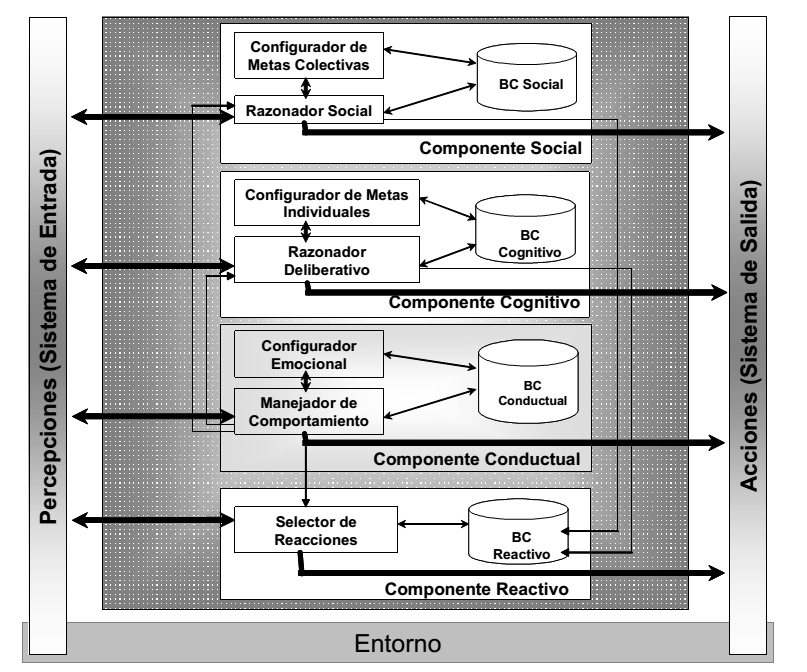
\includegraphics[width=6cm]{ilustraciones/componentes-masoes-individual}
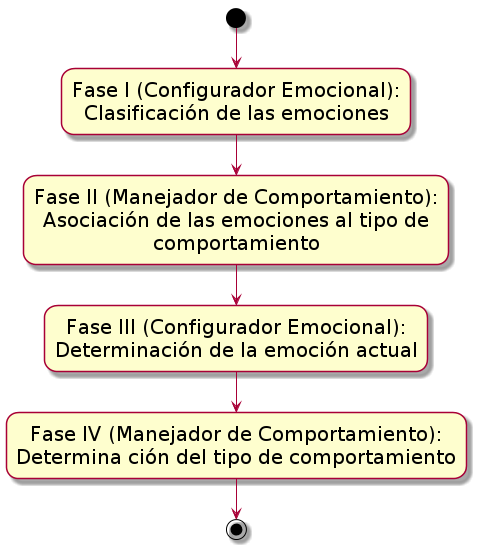
\includegraphics[width=4cm]{ilustraciones/componente-conductual}
\end{frame}

\begin{frame}
\frametitle{MASOES}
\framesubtitle{Modelo Afectivo de MASOES}
\centering
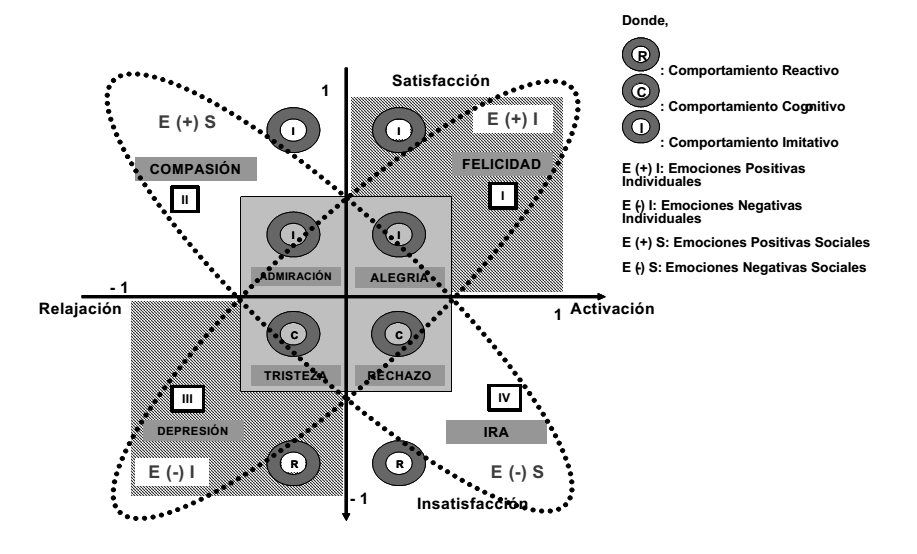
\includegraphics[width=9cm]{ilustraciones/modelo-afectivo}
\end{frame}

\begin{frame}
\frametitle{MASOES}
\framesubtitle{Reglas de Priorización de Comportamientos}
\begin{table}[!ht]
\centering
\scriptsize
\begin{tabular}{ll}
\hline
\textbf{Regla 1:} & Si el \textit{Estado Emocional} es \textit{Positivo} \\
& entonces priorizar \textit{Comportamiento Imitativo} \\
\textbf{Regla 2:} & Sino Si el \textit{Estado Emocional} es \textit{Ligeramente Negativo} \\
& entonces priorizar \textit{Comportamiento Cognitivo} \\
\textbf{Regla 3:} & Sino Si el \textit{Estado Emocional} es \textit{Altamente Negativo} \\
& entonces priorizar \textit{Comportamiento Reactivo} \\
\hline
\end{tabular}
\end{table}
\end{frame}

\section{Propuesta}

\begin{frame}
\frametitle{Propuesta}
\begin{itemize}
\item Frente a lo expuesto, el presente trabajo
propone una implementación del modelo afectivo de MASOES sobre un sistema
multiagente, con la finalidad de brindar un entorno para la interacción entre los
procesos emocionales y las diferentes funciones de un agente.
\item Además, se aplicó lo implementado sobre casos de estudio utilizando simulaciones para
generar emociones a nivel individual y colectivo, y se comparan los resultados a
nivel de implementación con los obtenidos a nivel de diseño.
\end{itemize}
\end{frame}

\begin{frame}
\frametitle{Propuesta}
\framesubtitle{Aspectos Arquitecturales}
\begin{columns}
\column{0.5\textwidth}
\textbf{JADE}\\
\textbf{Java Agent
DEvelopment}, uno de los marcos de trabajo con paradigma de POA (\textbf{Programación Orientada a Agentes})
más populares, implementado en el lenguaje de programación Java
\column{0.5\textwidth}
\textbf{FIPA}\\
\textbf{Foundation for Intelligent Physical Agents},
las cuales representan una colección de normas que tienen como objetivo promover la interoperabilidad
de agentes heterogéneos y los servicios que pueden representar
\end{columns}
\end{frame}

\begin{frame}
\frametitle{Propuesta}
\framesubtitle{Aspectos Arquitecturales}
\centering
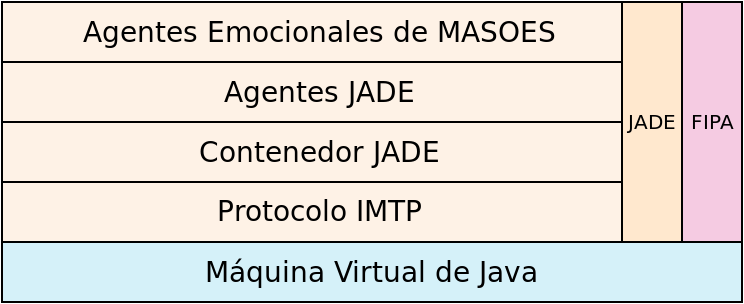
\includegraphics[width=6cm]{ilustraciones/arquitectura}
\vfill
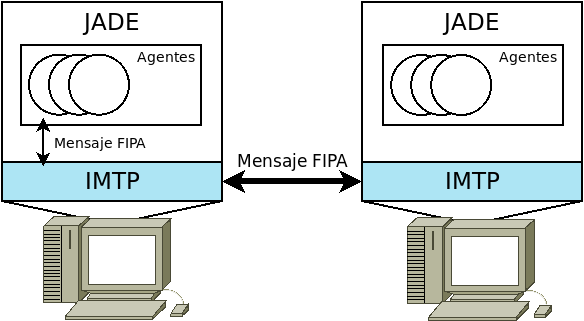
\includegraphics[width=6cm]{ilustraciones/comunicacion-entre-hosts}
\end{frame}

\begin{frame}
\frametitle{Aspectos Propuestos a Nivel Individual}
\framesubtitle{Propuesta de Una Ontología Para MASOES}
\begin{columns}
\column{0.5\textwidth}
\centering
\tiny
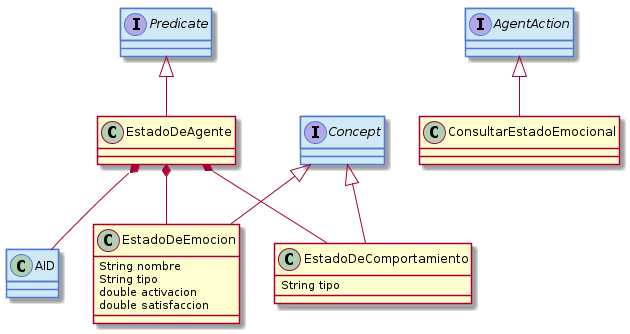
\includegraphics[width=5cm]{ilustraciones/ontologia-masoes-estado}
\\
Acción Consultar Estado del Agente
\column{0.5\textwidth}
\centering
\tiny
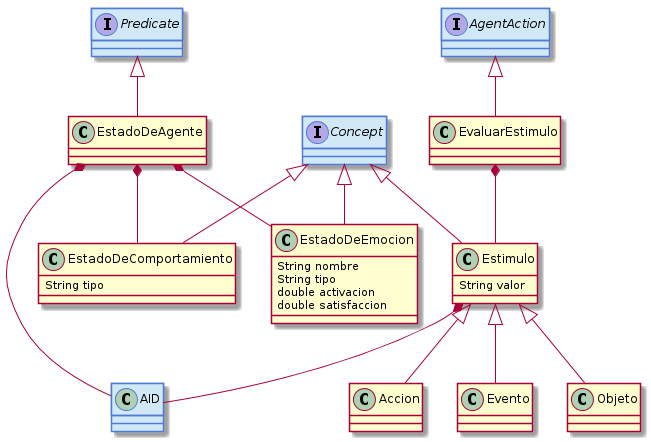
\includegraphics[width=5cm]{ilustraciones/ontologia-masoes-estimulo}
\\
Acción Evaluar Estímulo
\end{columns}
\end{frame}

\begin{frame}
\frametitle{Aspectos Propuestos a Nivel Individual}
\framesubtitle{Diseño del Agente Emocional}
\centering
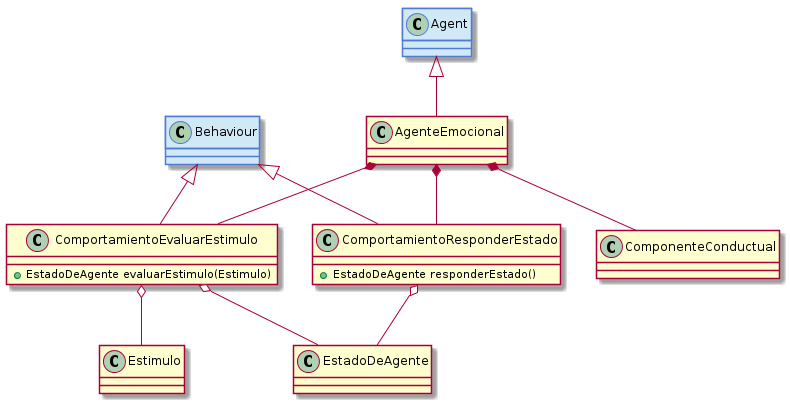
\includegraphics[width=7cm]{ilustraciones/diseno-nivel-individual}
\end{frame}

\begin{frame}
\frametitle{Aspectos Propuestos a Nivel Individual}
\framesubtitle{Diseño del Componente Conductual}
\centering
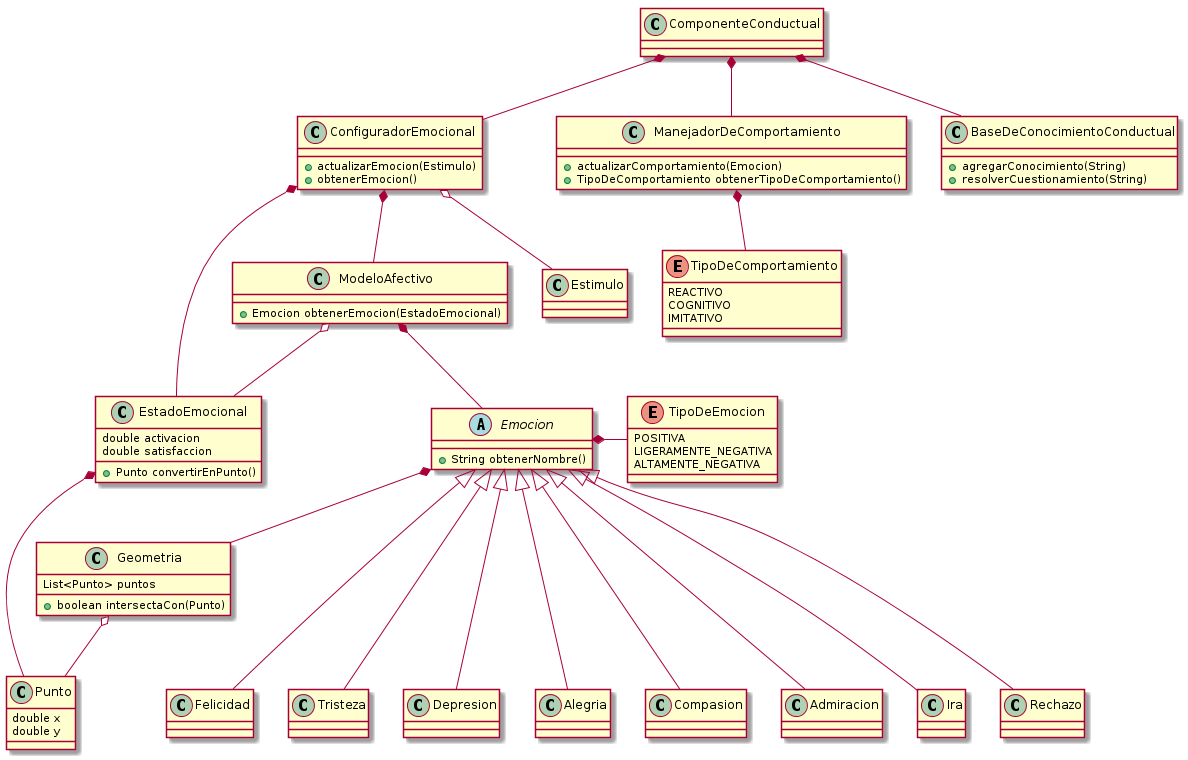
\includegraphics[width=9cm]{ilustraciones/diseno-componente-conductual}
\end{frame}

\begin{frame}
\frametitle{Componente Conductual}
\framesubtitle{Procesamiento de Estímulo}
\centering
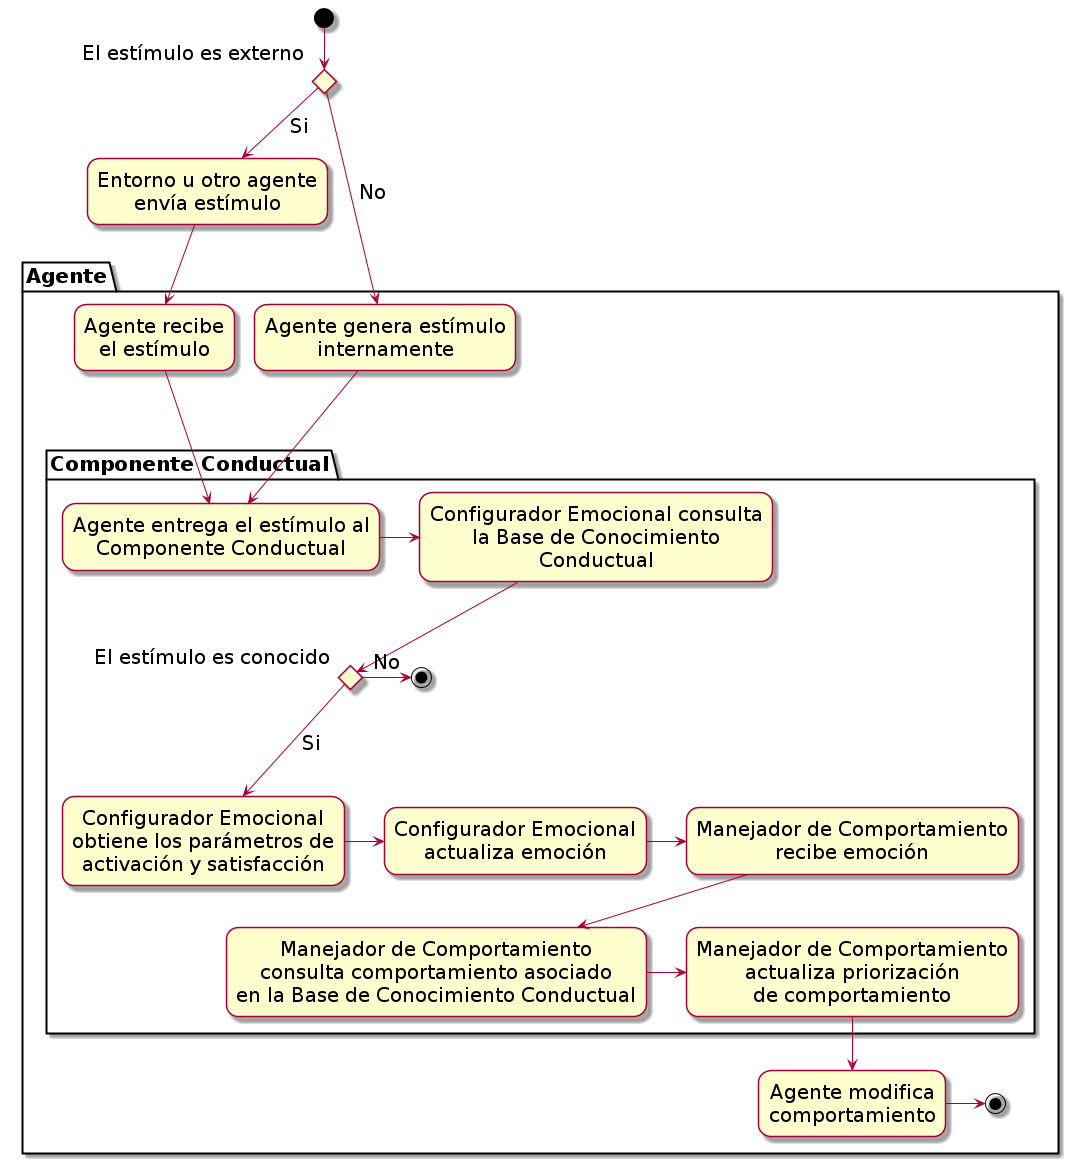
\includegraphics[width=6cm]{ilustraciones/procesamiento-estimulo}
\end{frame}

\begin{frame}
\frametitle{Aspectos Propuestos a Nivel Colectivo}
\framesubtitle{Cálculo de la Emoción Social}
\begin{exampleblock}{Emoción Social}
$ES(Ag) = \{EC(Ag), m(Ag), \sigma(Ag)\}$
\end{exampleblock}

Donde $Ag$ representa al grupo de agentes en estudio, $EC(Ag)$ se refiere a la
emoción central exhibida por el grupo de agentes, $m(Ag)$ es el estado emocional
más alejado de la $EC$, $\sigma(Ag)$ representa la dispersión emocional entorno
a la $EC$.
\end{frame}

\begin{frame}
\frametitle{Aspectos Propuestos a Nivel Colectivo}
\framesubtitle{Cálculo de la Emoción Social}
\begin{exampleblock}{Emoción Central}
$EC(Ag) = (\bar A(Ag), \bar S(Ag))$
\end{exampleblock}

\begin{exampleblock}{Promedio de la Activación}
$\bar A(Ag)=\frac{\sum_{i=1}^n A_i}{n}, \forall ag_i \in Ag$ \\
\end{exampleblock}

\begin{exampleblock}{Promedio de la Satisfacción}
$\bar S(Ag)=\frac{\sum_{i=1}^n S_i}{n}, \forall ag_i \in Ag$
\end{exampleblock}

\end{frame}

\begin{frame}
\frametitle{Aspectos Propuestos a Nivel Colectivo}
\framesubtitle{Cálculo de la Emoción Social}
\begin{exampleblock}{Distancia Máxima}
$ m(Ag) = (m_A(Ag), m_S(Ag))$
\end{exampleblock}

\begin{exampleblock}{Distancia Máxima de la Activación}
$m_A(Ag) = max\left(\sqrt{(A_i - \bar A(Ag))^2}\right), \forall ag_i \in Ag$
\end{exampleblock}

\begin{exampleblock}{Distancia Máxima de la Satisfacción}
$m_S(Ag) = max\left(\sqrt{(S_i - \bar S(Ag))^2}\right), \forall ag_i \in Ag$
\end{exampleblock}

\end{frame}

\begin{frame}
\frametitle{Aspectos Propuestos a Nivel Colectivo}
\framesubtitle{Cálculo de la Emoción Social}
\begin{exampleblock}{Dispersión Emocional}
$ \sigma(Ag) = (\sigma_A(Ag), \sigma_S(Ag))$
\end{exampleblock}

\begin{exampleblock}{Dispersión Emocional de la Activación}
$\sigma_A(Ag) = \sqrt{\frac{\sum_{i=1}^n(A_i - \bar A(Ag))^2}{n}},  \forall ag_i \in Ag$
\end{exampleblock}

\begin{exampleblock}{Dispersión Emocional de la Satisfacción}
$  \sigma_S(Ag) = \sqrt{\frac{\sum_{i=1}^n(S_i - \bar S(Ag))^2}{n}},  \forall ag_i \in Ag$
\end{exampleblock}
\end{frame}

\section{Casos de Estudio}

\begin{frame}
\frametitle{Casos de Estudio}
\framesubtitle{Estímulos Asociados al Usuario Registrado Propuestos para los Casos de Estudio de Wikipedia}
\begin{table}[!ht]
\centering
\scriptsize
\begin{tabular}{lll}
\hline
Estímulo & $P_a$ & $P_s$ \\
\hline\hline
\multicolumn{3}{l}{\textbf{Aumento de Reputación}} \\ \hline\hline
Artículo Nuevo & 0.05 & 0.05  \\ \hline
Nueva Edición & 0.03 & 0.04  \\ \hline
Artículo Sobresaliente & 0.08 & 0.08  \\ \hline\hline
\multicolumn{3}{l}{\textbf{Decremento de Reputación}} \\ \hline\hline
Guerra de Ediciones & -0.08 & -0.08 \\ \hline
Artículo Borrado & -0.06 & -0.06  \\ \hline
Artículo Modificado & -0.02 & -0.03  \\
\hline
\end{tabular}
\end{table}
\end{frame}

\begin{frame}
\frametitle{Caso de Estudio 1: Emociones a Nivel Social}
\framesubtitle{Escenario 1: Baja Dispersión Emocional y Bajo Número de Agentes}
\begin{columns}
\column{0.5\textwidth}
\tiny
\centering
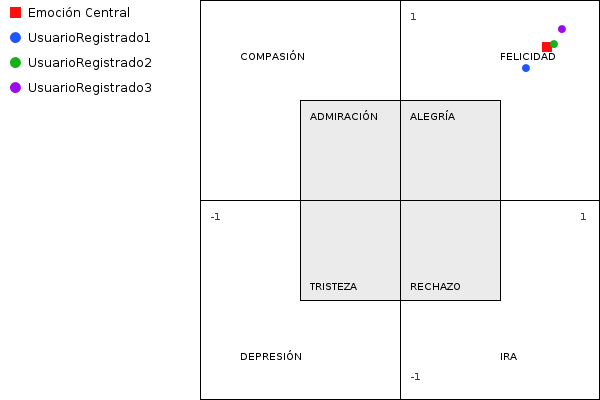
\includegraphics[width=5cm]{ilustraciones/caso1escenario1-emocioncentral}
\column{0.5\textwidth}
\tiny
\centering
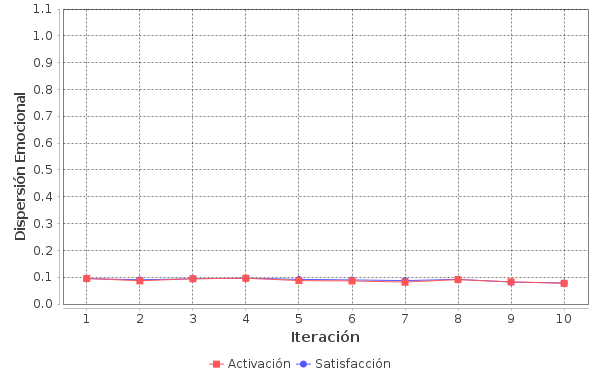
\includegraphics[width=5cm]{ilustraciones/caso1escenario1-dispersionemocional}
\end{columns}
\end{frame}

\begin{frame}
\frametitle{Caso de Estudio 1: Emociones a Nivel Social}
\framesubtitle{Escenario 2: Alta Dispersión Emocional y Bajo Número de Agentes}
\begin{columns}
\column{0.5\textwidth}
\tiny
\centering
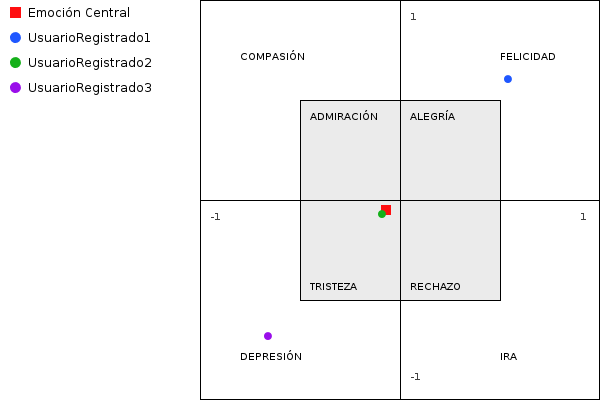
\includegraphics[width=5cm]{ilustraciones/caso1escenario2-emocioncentral}
\column{0.5\textwidth}
\tiny
\centering
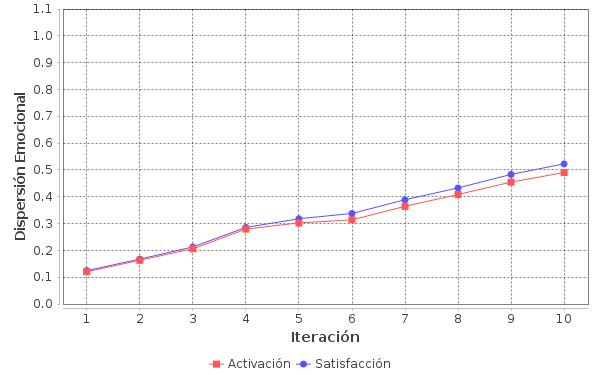
\includegraphics[width=5cm]{ilustraciones/caso1escenario2-dispersionemocional}
\end{columns}
\end{frame}

\begin{frame}
\frametitle{Caso de Estudio 1: Emociones a Nivel Social}
\framesubtitle{Escenario 3: Baja Dispersión Emocional y Alto Número de Agentes}
\begin{columns}
\column{0.5\textwidth}
\tiny
\centering
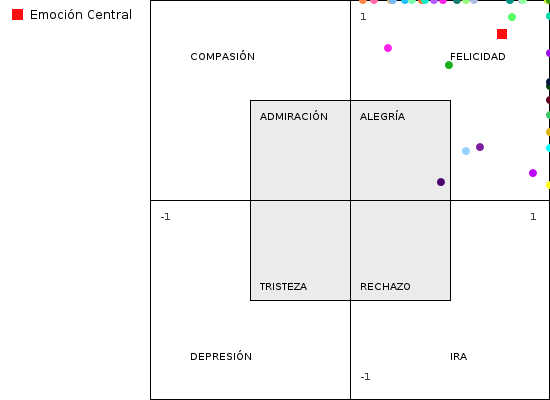
\includegraphics[width=5cm]{ilustraciones/caso1escenario3-emocioncentral-final}
\column{0.5\textwidth}
\tiny
\centering
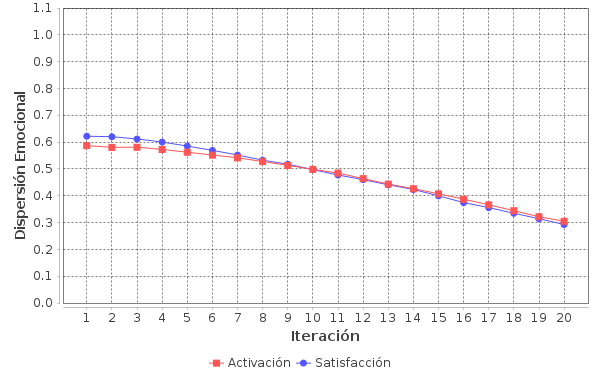
\includegraphics[width=5cm]{ilustraciones/caso1escenario3-dispersionemocional}
\end{columns}
\end{frame}

\begin{frame}
\frametitle{Caso de Estudio 1: Emociones a Nivel Social}
\framesubtitle{Escenario 4: Alta Dispersión Emocional y Alto Número de Agentes}
\begin{columns}
\column{0.5\textwidth}
\tiny
\centering
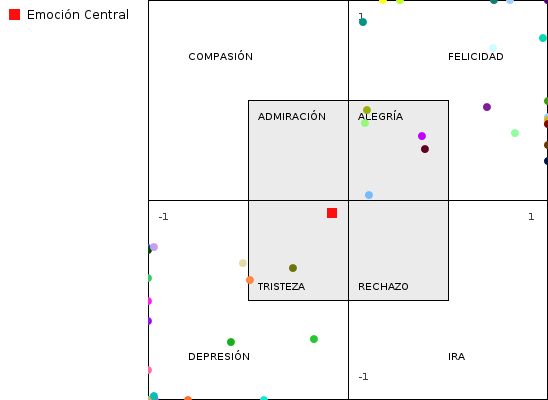
\includegraphics[width=5cm]{ilustraciones/caso1escenario4-emocioncentral-final}
\column{0.5\textwidth}
\tiny
\centering
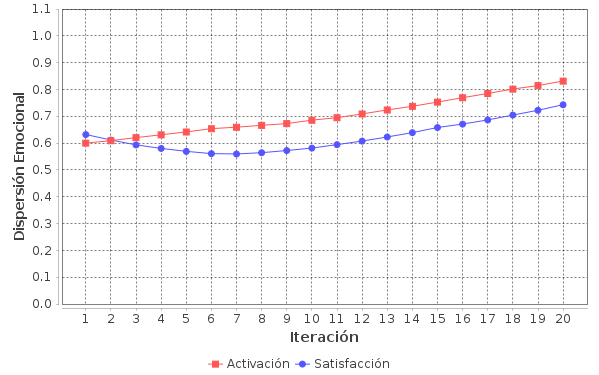
\includegraphics[width=5cm]{ilustraciones/caso1escenario4-dispersionemocional}
\end{columns}
\end{frame}

\begin{frame}
\frametitle{Caso de Estudio 2: Emociones a Nivel Individual}
\framesubtitle{Escenario 1: Grado de Satisfacción Alto y Activación Alto, Medio y Bajo}
\begin{columns}
\column{0.5\textwidth}
\tiny
\centering
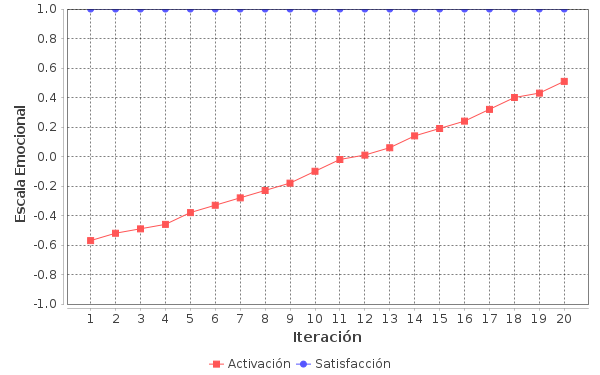
\includegraphics[width=5cm]{ilustraciones/caso2escenerio1-estado-emocional-colaborador1}
\column{0.5\textwidth}
\tiny
\centering
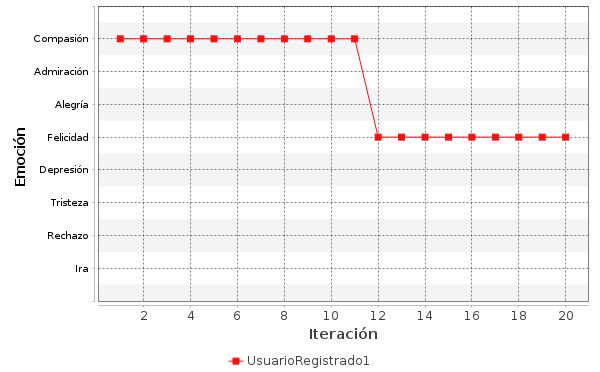
\includegraphics[width=5cm]{ilustraciones/caso2escenerio1-modificacion-de-emociones}

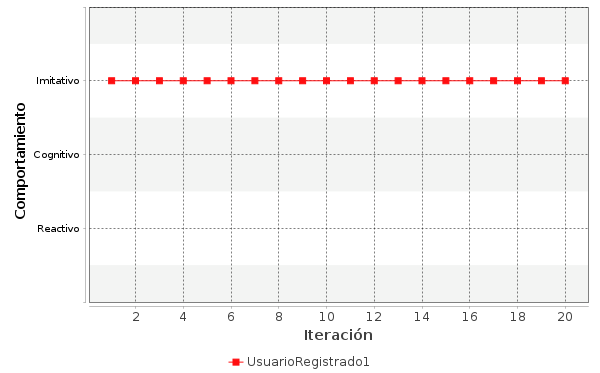
\includegraphics[width=5cm]{ilustraciones/caso2escenerio1-modificacion-de-comportamiento}
\end{columns}
\end{frame}

\begin{frame}
\frametitle{Caso de Estudio 2: Emociones a Nivel Individual}
\framesubtitle{Escenario 2: Grado de Satisfacción y Activación Medio y Bajo}
\begin{columns}
\column{0.5\textwidth}
\tiny
\centering
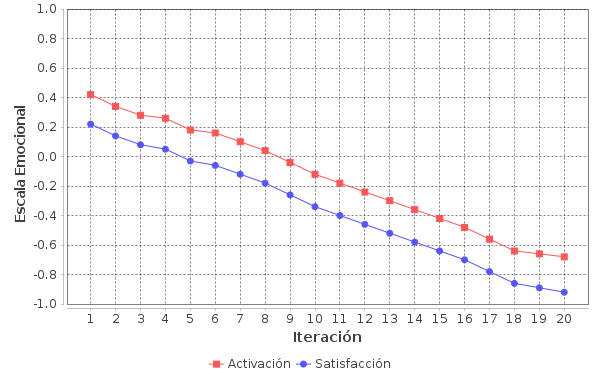
\includegraphics[width=5cm]{ilustraciones/caso2escenerio2-estado-emocional-colaborador1}
\column{0.5\textwidth}
\tiny
\centering
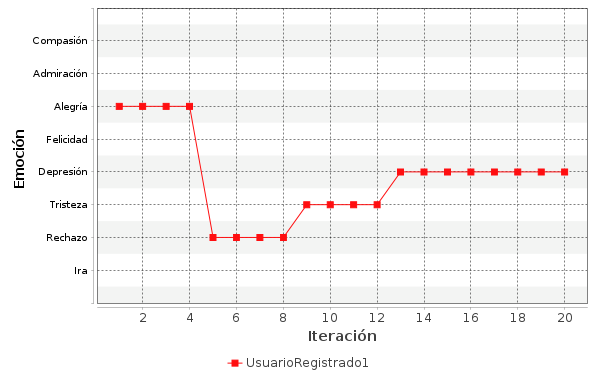
\includegraphics[width=5cm]{ilustraciones/caso2escenerio2-modificacion-de-emociones}

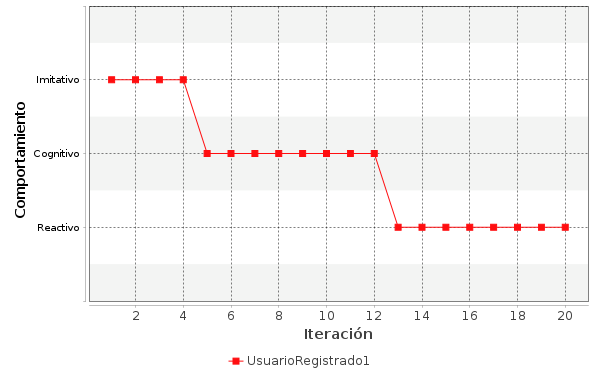
\includegraphics[width=5cm]{ilustraciones/caso2escenerio2-modificacion-de-comportamiento}
\end{columns}
\end{frame}

\DoBlueBackgroundTitle{Demostración}

\section{Conclusiones}
\begin{frame}
\frametitle{Conclusiones}
\begin{itemize}
  \item Se abordó la implementación del modelo afectivo
  propuesto en MASOES, y por ende su componente conductual.
	\item Se propone el cálculo de
  la Emoción Social de un grupo de agentes.
  \item Los resultados obtenidos demuestran que la implementación cumple
  con lo requerido en MASOES, tanto a nivel individual como colectivo.
  \item Se pudo comprobar que la emoción central es más válida a medida que la dispersión
  emocional es más cercana a cero, ya que se trata de un conjunto de agentes que tienen emociones muy parecidas (homogéneas).
\end{itemize}
\end{frame}

\begin{frame}
\frametitle{Conclusiones}
\begin{itemize}
  \item Este trabajo proporciona un marco de trabajo el cual se puede seguir extendiendo,
  para simular cualquier tipo de sistema emergente y auto-organizado modelado con MASOES.
  \item Se propone una ontología de
  comunicación para MASOES, específicamente para agentes estandarizados FIPA, con ella
  es posible comunicar los agentes emocionales entre sí o con otros tipos de agentes.
\end{itemize}
\end{frame}

\section{Publicaciones}
\begin{frame}
\frametitle{Publicaciones}
\begin{itemize}
\item Implementación de un Modelo Afectivo para MASOES. Latin American Journal of Computing, Escuela Politécnica Nacional
Quito-Ecuador. Aceptado para Publicación, 2017.
\item Conferencia: Modelos Emocionales Dimensionales. VIII Jornadas de Ingeniería de Sistemas Informáticos y de Computación (JISIC) NOV/2017, Escuela Politécnica Nacional
Quito-Ecuador.
\item Verificación a Nivel de Implementación de un Modelo Afectivo Para la Arquitectura Multiagente Para Sistemas Emergentes y Auto-organizados (MASOES). Reporte Técnico por enviar a Revista para evaluación, 2017.
\end{itemize}
\end{frame}

\section{Trabajos Futuros}
\begin{frame}
\frametitle{Trabajos Futuros}
\begin{itemize}
  \item Se podría implementar otros componentes individuales de la arquitectura de MASOES,
  como son, los componentes Cognitivo, Reactivo y Social.
	\item Adaptar a otros componentes de MASOES la Base de Conocimiento Colectivo .
  \item Proponer un cálculo de emoción social,
  que pueda dar como resultado más de una emoción central, esto, basado en las agrupaciones de estados emocionales
  que puedan emerger en el grupo de agentes.
\end{itemize}
\end{frame}

\DoBlueBackgroundTitle{Preguntas}

\ThankYouFrame

\end{document}
